W ramach etapu podziału siatki na $m \cdot k$ obszarów wyróżniam konwersje pliku graficznego na graf, redukcje rozmiaru grafu,
podzielenie zredukowanego grafu oraz przywrócenie grafu do początkowego rozmiaru wraz z wprowadzeniem optymalizacji podziału
(wyrównanie pól i zmniejszenie długości granic pomiędzy partycjami).

\subsubsection{Konwersja pliku graficznego na graf i redukcja obszarów niepodzielnych}

Pierwszą częścią algorytmu jest tworzenie grafu, na podstawie siatki, która dostarczana jest jako dana wejściowa.
Siatka jest w formie pliku graficznego.
Przykład takiego pliku przedstawiony jest na rysunku \ref{im:input}.
Jeden piksel na siatce reprezentuje jeden wierzchołek w grafie, na którym dokonywane będzie partycjonowanie.
Kolor piksela decyduje o tym, jakiego typu wierzchołkiem będzie dany piksel oraz do jakiego typu obszaru należy.
Wierzchołki, które są tego samego koloru oraz są do siebie sąsiednie przyporządkowywane są do tego samego obszaru.
Żółte piksele interpretowane są jako wierzchołki obszarów niepodzielnych, natomiast czerwone piksele
jako wierzchołki obszarów wyłączonych z obliczeń, białe piksele to wierzchołki zwyczajne.
Obszary wyłączone z obliczeń mogą być używane do zaznaczenia fragmentów siatki, na których wiemy, że symulacja
nie będzie miała miejsca.
Przykładowo mogą być to ściany budynku lub pomieszczenia, które są wyłączone z symulacji.
Obszary niepodzielne to obszary, o których z jakiś powodów wiemy, że nie powinny być podzielone na partycje.
Na przykład mogą być to wejścia do budynków.
Przynależność wierzchołków do konkretnych grup wpływa na ich parametry w grafie, jak na przykład waga.
Może również prowadzić do tego, że nie pojawią się na grafie.
Ta część algorytmu, choć stosunkowo mało skomplikowana, jest kluczową dla niniejszej pracy.
W związku z tym, że autorzy artykułu \cite{1364754} nie zawarli informacji w jakiej formie dostarczany był
wejściowy graf, ta część algorytmu była zrealizowana w całości przeze mnie.
Efekt zamiany siatki na graf widoczny jest rysunku \ref{im:input2}.

\begin{figure}[h]
    \centering
    \fbox{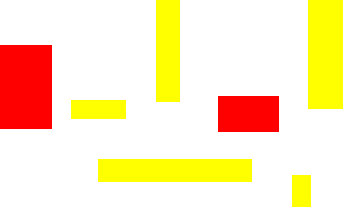
\includegraphics[width=0.6\linewidth]{images/grid1}}
    \caption{Obrazek, który reprezentuje strukturę siatki do podziału. Żółte obszary to obszary niepodzielne, czerwone to
    te wyłączone z obliczeń, białe to zwykłe przez które przechodzić będą granice podziału.}
    \label{im:input}
\end{figure}

Algorytm iteruje po pikselach obrazka wejściowego i na podstawie ich koloru tworzy wierzchołki w grafie oraz buduje zbiory
obszarów niepodzielnych oraz wyłączonych z obliczeń.
W zbiorach przechowywane są numery wierzchołków.
Na początku każda krawędź pomiędzy wierzchołkami ma wagę $1$.
Zwykłe wierzchołki oraz wierzchołki obszarów niepodzielnych otrzymują wagę $1$.
Wierzchołki obszarów wyłączonych z obliczeń mogą mieć przyporządkowaną wagę $0$ lub nie być mapowane na wierzchołki w grafie,
tworząc puste przestrzenie między wierzchołkami.
Każdy wierzchołek w grafie ma parametr, który określa jakim typem obszaru jest.
Kolejnym etapem jest redukcja obszarów niepodzielnych do pojedynczych wierzchołków.
Każdy obszar niepodzielny zamieniany jest na wierzchołek o wadze równej sumie wag wierzchołków tego obszaru.
Od teraz wierzchołki, które reprezentują obszary niepodzielne, nie są więcej rozróżniane jako obszary niepodzielne -
stają się zwykłymi
wierzchołkami.
Ten proces przedstawiony jest na rysunku \ref{im:indivisible}.

W dalszych częściach algorytmu następuje partycjonowanie oraz przemieszczanie wierzchołków między partycjami.
Wszystkie te operacje będą następowały na grafie z przynajmniej zredukowanymi obszarami niepodzielnymi.
Do tych operacji graf może być zredukowany bardziej, nigdy mniej.
W ten sposób obszary niepodzielne zawsze traktowane są jako całość, nigdy nie zostaną odłączone od nich żadne pojedyncze
wierzchołki.
Wierzchołki wyłączone z obliczeń mają wagę $0$, ponieważ później wykorzystywane algorytmy do partycjonowania grafu operują
głównie na parametrze wagi wierzchołków.
Waga wierzchołka w zredukowanym grafie symbolizuje ile wierzchołków z grafu początkowego reprezentuje, a to ma wpływ
na balansowanie pól obszarów.
Chcemy, aby partycje były równe pod względem wierzchołków, na których będą występować obliczenia.
Ustawianie wagi na $0$ oznacza, że taki wierzchołek nie jest brany pod uwagę w wyrównywaniu pól obszarów, jest
bez znaczenia dla algorytmu, może być dowolnie przemieszczany pomiędzy partycjami.

\vspace{8mm}

\begin{figure}[h]
\centering
\begin{subfigure}{.2\textwidth}
    \centering
    \fbox{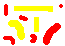
\includegraphics[width=0.6\linewidth]{images/strange7}}
    \caption[short]{}
\end{subfigure}%
\begin{subfigure}{.38\textwidth}
    \centering
    \fbox{
\includegraphics[width=0.8\linewidth]{images/rm/2}}
    \caption[short]{}
\end{subfigure}%
\begin{subfigure}{.38\textwidth}
    \centering
    \fbox{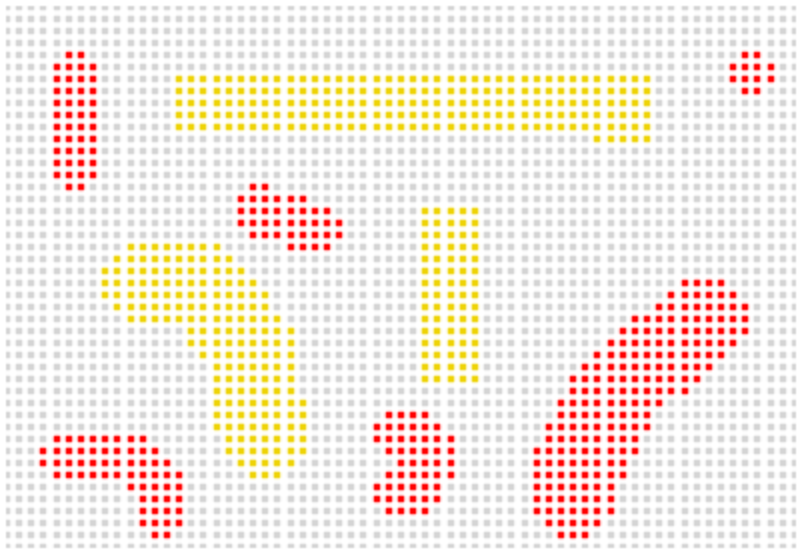
\includegraphics[width=0.8\linewidth]{images/rm/1}}
    \caption[short]{}
\end{subfigure}
\caption{Obrazek (a) przedstawia obrazek wejściowy w rzeczywistym rozmiarze. Obrazki (b) oraz (c) przedstawiają
powstały graf. Obrazek (b) przedstawia sposób podejścia do obszarów wyłączonych z obliczeń, gdzie nie tworzone są
odwzorowujące je wierzchołki, obrazek (c) pokazuje podejście gdzie w ich miejsce tworzone są wierzchołki z wagą $0$.
Dla czytelności wierzchołki zwykłe zostały oznaczone kolorem szarym. }
\label{im:input2}
\end{figure}

\begin{figure}[h]
\centering
\begin{subfigure}{.5\textwidth}
    \centering
    \fbox{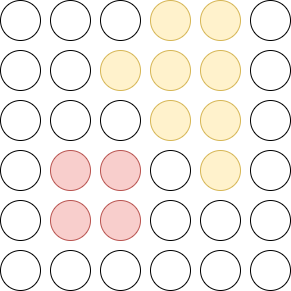
\includegraphics[width=0.6\linewidth]{images/in/1}}
    \caption[short]{}
\end{subfigure}
\begin{subfigure}{.5\textwidth}
    \centering
    \fbox{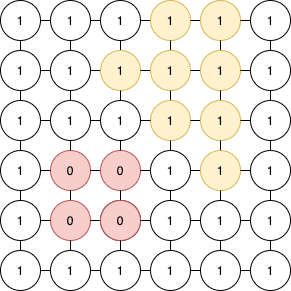
\includegraphics[width=0.6\linewidth]{images/in/2}}
    \caption[short]{}
\end{subfigure}%
\begin{subfigure}{.5\textwidth}
    \centering
    \fbox{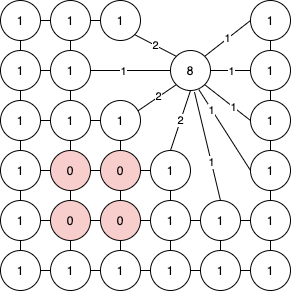
\includegraphics[width=0.6\linewidth]{images/in/3}}
    \caption[short]{}
\end{subfigure}
\begin{subfigure}{.5\textwidth}
    \centering
    \fbox{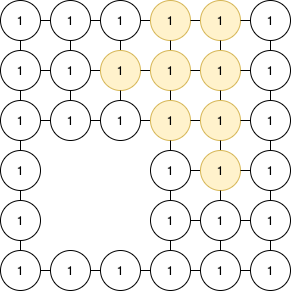
\includegraphics[width=0.6\linewidth]{images/in/4}}
    \caption[short]{}
\end{subfigure}%
\begin{subfigure}{.5\textwidth}
    \centering
    \fbox{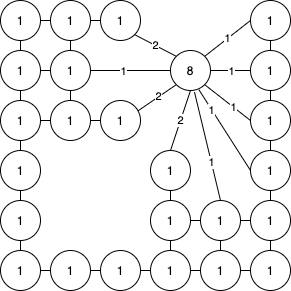
\includegraphics[width=0.6\linewidth]{images/in/5}}
    \caption[short]{}
\end{subfigure}
\caption{Obrazek (a) to wejściowa siatka.
Obszary niepodzielne są żółte, natomiast wyłączona z obliczeń czerwone.
Obrazek (b) oraz (d) pokazują siatkę tuż po konwersji na graf wedle dwóch sposobów.
Sposób (b) nadaje wierzchołkom na obszarach wyłączonych z obliczeń wagę $0$, natomiast sposób (d) usuwa wierzchołki obszarów
wyłączonych z obliczeń.
Na wierzchołkach zaznaczona jest waga.
Można zaobserwować wagę $1$ dla wierzchołków zwykłych i tych budujących obszary niepodzielne.
Na tym etapie wszystkie krawędzie mają wagę $1$. Obrazek (c) oraz (e) przedstawiają ten sam graf po redukcji obszarów
niepodzielnych, odpowiednio z kroku (b) oraz (d).
Wierzchołek, do którego został zredukowany obszar niepodzielny otrzymuje powiększoną wagę, równą sumie wag wierzchołków, które
redukuje. Niektóre krawędzie, które zastąpiły dwie krawędzie, zyskują sumę wag tych krawędzi równą $2$.}
\label{im:indivisible}
\end{figure}

\FloatBarrier


